\documentclass[11pt, a4paper]{article}
\usepackage{pdfpages}
\usepackage{parallel}
\usepackage[T2A]{fontenc}
%\usepackage{ucs}
\usepackage[utf8]{inputenc}
\usepackage[english,russian]{babel}
\usepackage{hyperref}
\usepackage{rotating}
\usepackage[inner=2cm,top=1.8cm,outer=2cm,bottom=2.3cm,nohead]{geometry}
%\usepackage{listings}
\usepackage{graphicx}
\usepackage{wrapfig}
\usepackage{longtable}
\usepackage{indentfirst}
\usepackage{array}
\usepackage{tikzsymbols}
\usepackage{soul}
\usepackage[ruled,vlined]{algorithm2e}
\usepackage{qrcode}
\counterwithout{figure}{section} 

\usepackage{url}
\makeatletter
\g@addto@macro{\UrlBreaks}{\UrlOrds}
\makeatother

\newcolumntype{P}[1]{>{\raggedright\arraybackslash}p{#1}}
\frenchspacing
%\usepackage{fixltx2e} %text sub- and superscripts
\usepackage{icomma} % коскі ў матэматычным рэжыме
%\PreloadUnicodePage{4}

\newcommand{\longpage}{\enlargethispage{\baselineskip}}
\newcommand{\shortpage}{\enlargethispage{-\baselineskip}}

\def\switchlang#1{\expandafter\csname switchlang#1\endcsname}
\def\switchlangbe{
\let\saverefname=\refname%
\def\refname{Літаратура}%
\def\figurename{Іл.}%
}
\def\switchlangru{
\let\saverefname=\refname%
\let\savefigurename=\figurename%
\def\refname{Литература}%
\def\figurename{Рис.}%
}
\def\switchlangen{
\let\saverefname=\refname%
\def\refname{References}%
\def\figurename{Fig.}%
}

\hyphenation{admi-ni-stra-tive}
\hyphenation{ex-pe-ri-ence}
\hyphenation{fle-xi-bi-li-ty}
\hyphenation{Py-thon}
\hyphenation{ma-the-ma-ti-cal}
\hyphenation{re-ported}
\hyphenation{imp-le-menta-tions}
\hyphenation{pro-vides}
\hyphenation{en-gi-neering}
\hyphenation{com-pa-ti-bi-li-ty}
\hyphenation{im-pos-sible}
\hyphenation{desk-top}
\hyphenation{elec-tro-nic}
\hyphenation{com-pa-ny}
\hyphenation{de-ve-lop-ment}
\hyphenation{de-ve-loping}
\hyphenation{de-ve-lop}
\hyphenation{da-ta-ba-se}
\hyphenation{plat-forms}
\hyphenation{or-ga-ni-za-tion}
\hyphenation{pro-gramming}
\hyphenation{in-stru-ments}
\hyphenation{Li-nux}
\hyphenation{sour-ce}
\hyphenation{en-vi-ron-ment}
\hyphenation{Te-le-pathy}
\hyphenation{Li-nux-ov-ka}
\hyphenation{Open-BSD}
\hyphenation{Free-BSD}
\hyphenation{men-ti-on-ed}
\hyphenation{app-li-ca-tion}

\def\progref!#1!{\texttt{#1}}
\renewcommand{\arraystretch}{2} %Іначай формулы ў матрыцы зліпаюцца з лініямі
\usepackage{array}

\def\interview #1 (#2), #3, #4, #5\par{

\section[#1, #3, #4]{#1 -- #3, #4}
\def\qname{LVEE}
\def\aname{#1}
\def\q ##1\par{{\noindent \bf \qname: ##1 }\par}
\def\a{{\noindent \bf \aname: } \def\qname{L}\def\aname{#2}}
}

\def\interview* #1 (#2), #3, #4, #5\par{

\section*{#1\\{\small\rm #3, #4. #5}}
\ifx\ParallelWhichBox\undefined%
    \addcontentsline{toc}{section}{#1, #3, #4}%
\else%
\ifnum\ParallelWhichBox=0%
    \addcontentsline{toc}{section}{#1, #3, #4}%
\fi\fi%

\def\qname{LVEE}
\def\aname{#1}
\def\q ##1\par{{\noindent \bf \qname: ##1 }\par}
\def\a{{\noindent \bf \aname: } \def\qname{L}\def\aname{#2}}
}

\newcommand{\interviewfooter}[1]{
\vskip 1em
\noindent \textit{#1}
}

\AtEndDocument{\vfill\centering \qrcode{https://github.com/fiowro/mouses/blob/main/\jobname.pdf}}

\switchlang{ru}
\begin{document}

\title{1985 "--- Logitech С7 mouse}
\date{}
\maketitle
\selectlanguage{russian}
Мышь Logitech C7 была выпущена в 1985 году. Она стала первой мышью, выпущенной под брэндом Logitech \cite{timeline} и одновременно пробным шаром Logitech на ниве выпуска мышей для розничной продажи (до этого компания производила мышей для поставок ОЕМ). Отпускная цена C7 составляла всего \$100, что было заметно дешевле других оптомеханических мышей того времени. По-видимому именно это, наряду с удачной конструкцией, сделало мышь очень популярной среди конечных пользователей, несмотря на её заметную <<квадратность>> (рис. \ref{fig:LogitechC7Pic}).

\begin{figure}[h]
   \centering
    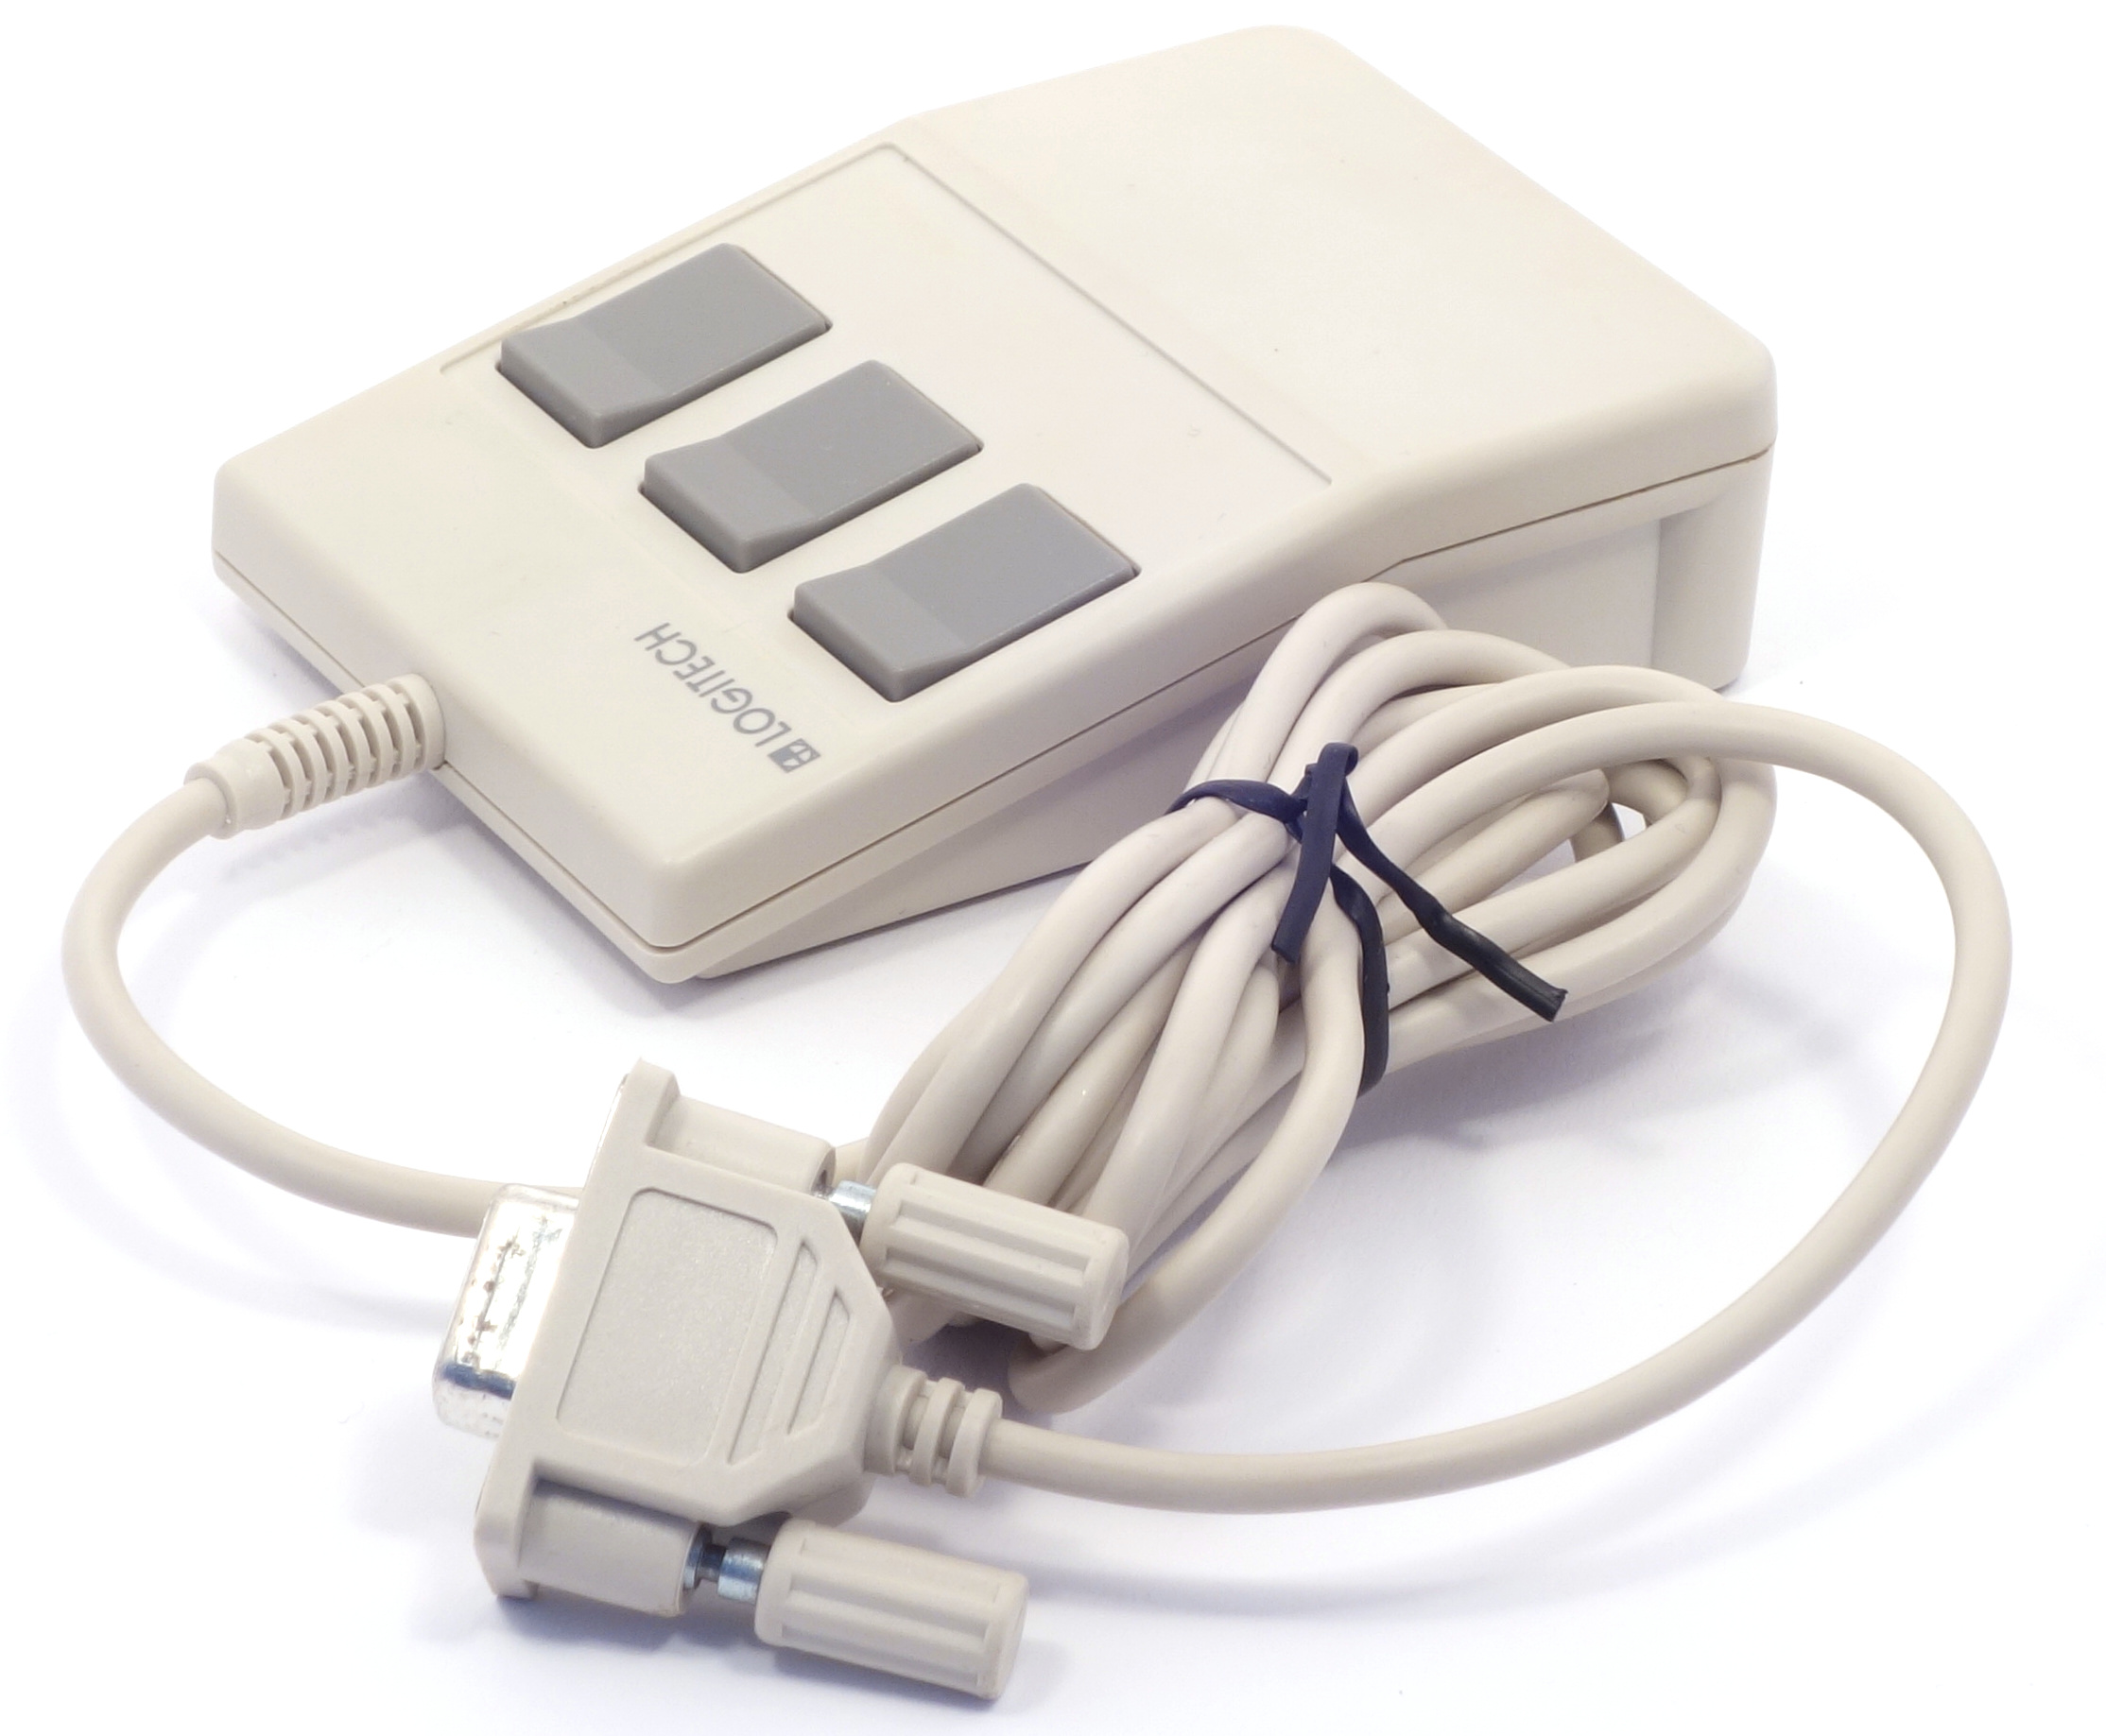
\includegraphics[scale=0.45]{1985_logitech_c7_mouse/pic_60.jpg}
    \caption{Logitech C7 mouse, вид спереди}
    \label{fig:LogitechC7Pic}
\end{figure}

В форме корпуса мыши прослеживается ощутимое сходство с более ранней моделью, LOGIMOUSE P5, созданной при участии известного швейцарского дизайнера Антуана Каэна. В С7 отказались от стогой призматической формы корпуса, предоставив пользователю горизональную площадку для опоры ладонью, а также слегка скруглённые ребра и углы. Узкие диагональные кнопки P5 уступили место значительно более удобным прмоугольным клавишам с большой площадью. Нижняя сторона сохранила еще больше сходства с P5: на ней также присутствуют четыре белые опоры с низким коэффициентом трения (на этот раз наклеенные на стенку корпуса, что вскоре станет повсеместно распространенным явлением) и съемное поворотное кольцо на защелках, позволяющее извлечь шар для чистки мыши (рис. \ref{fig:LogitechC7TopAndBottom}).

\begin{figure}[h]
    \centering
    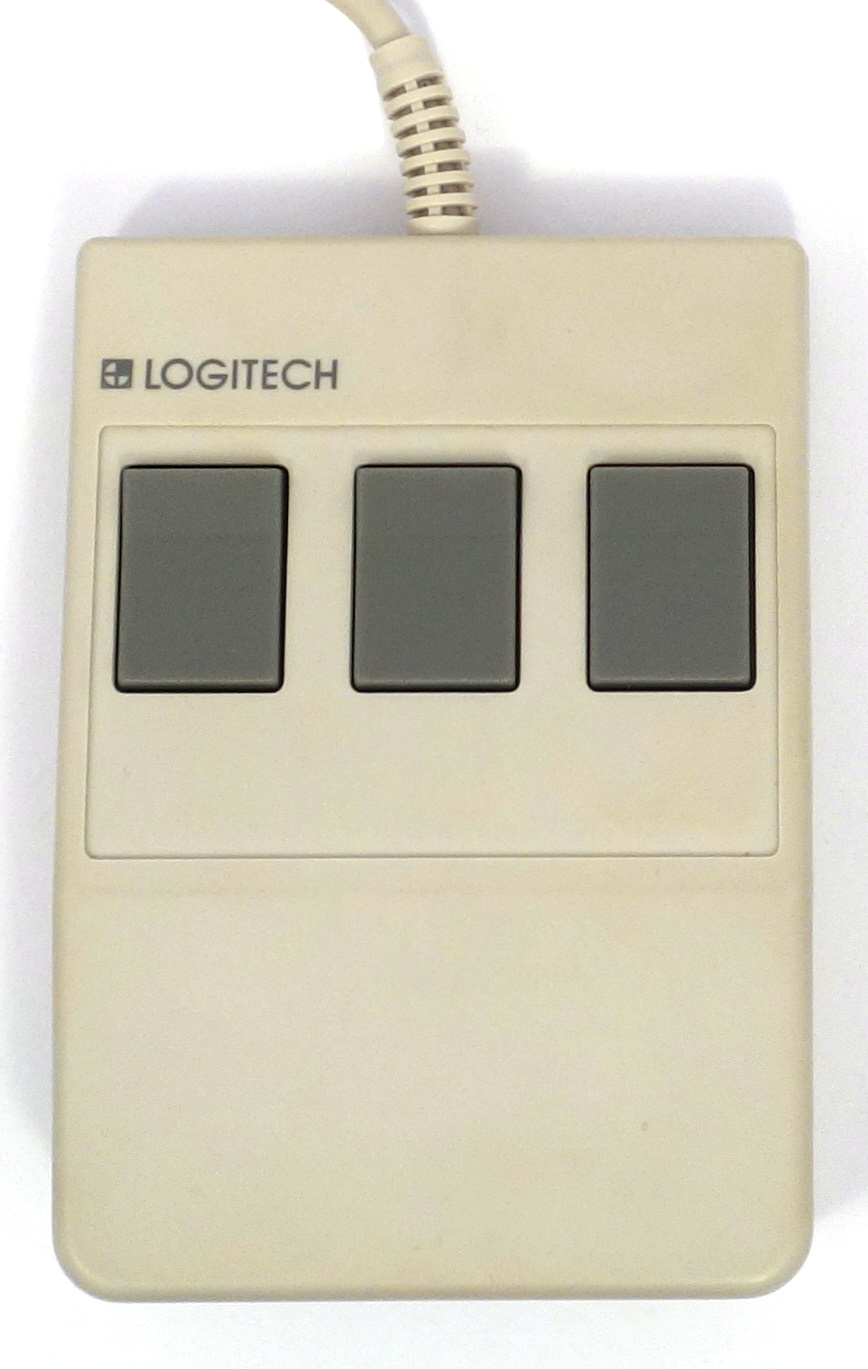
\includegraphics[scale=0.4]{1985_logitech_c7_mouse/top_30.jpg}
    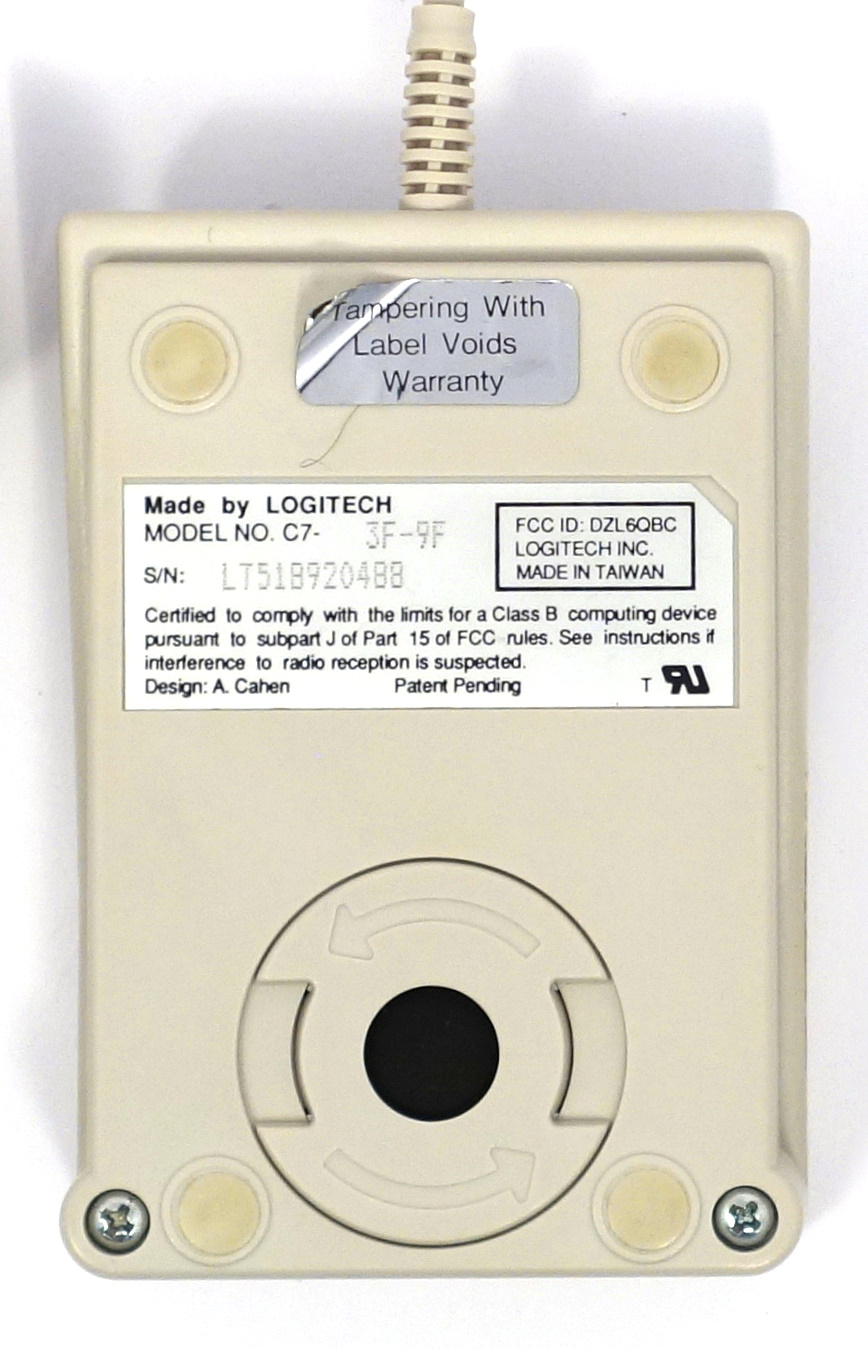
\includegraphics[scale=0.4]{1985_logitech_c7_mouse/bottom_30.jpg}
    \caption{Logitech C7 mouse, вид сверху и снизу}
    \label{fig:LogitechC7TopAndBottom}
\end{figure}

\begin{figure}[h]
    \centering
    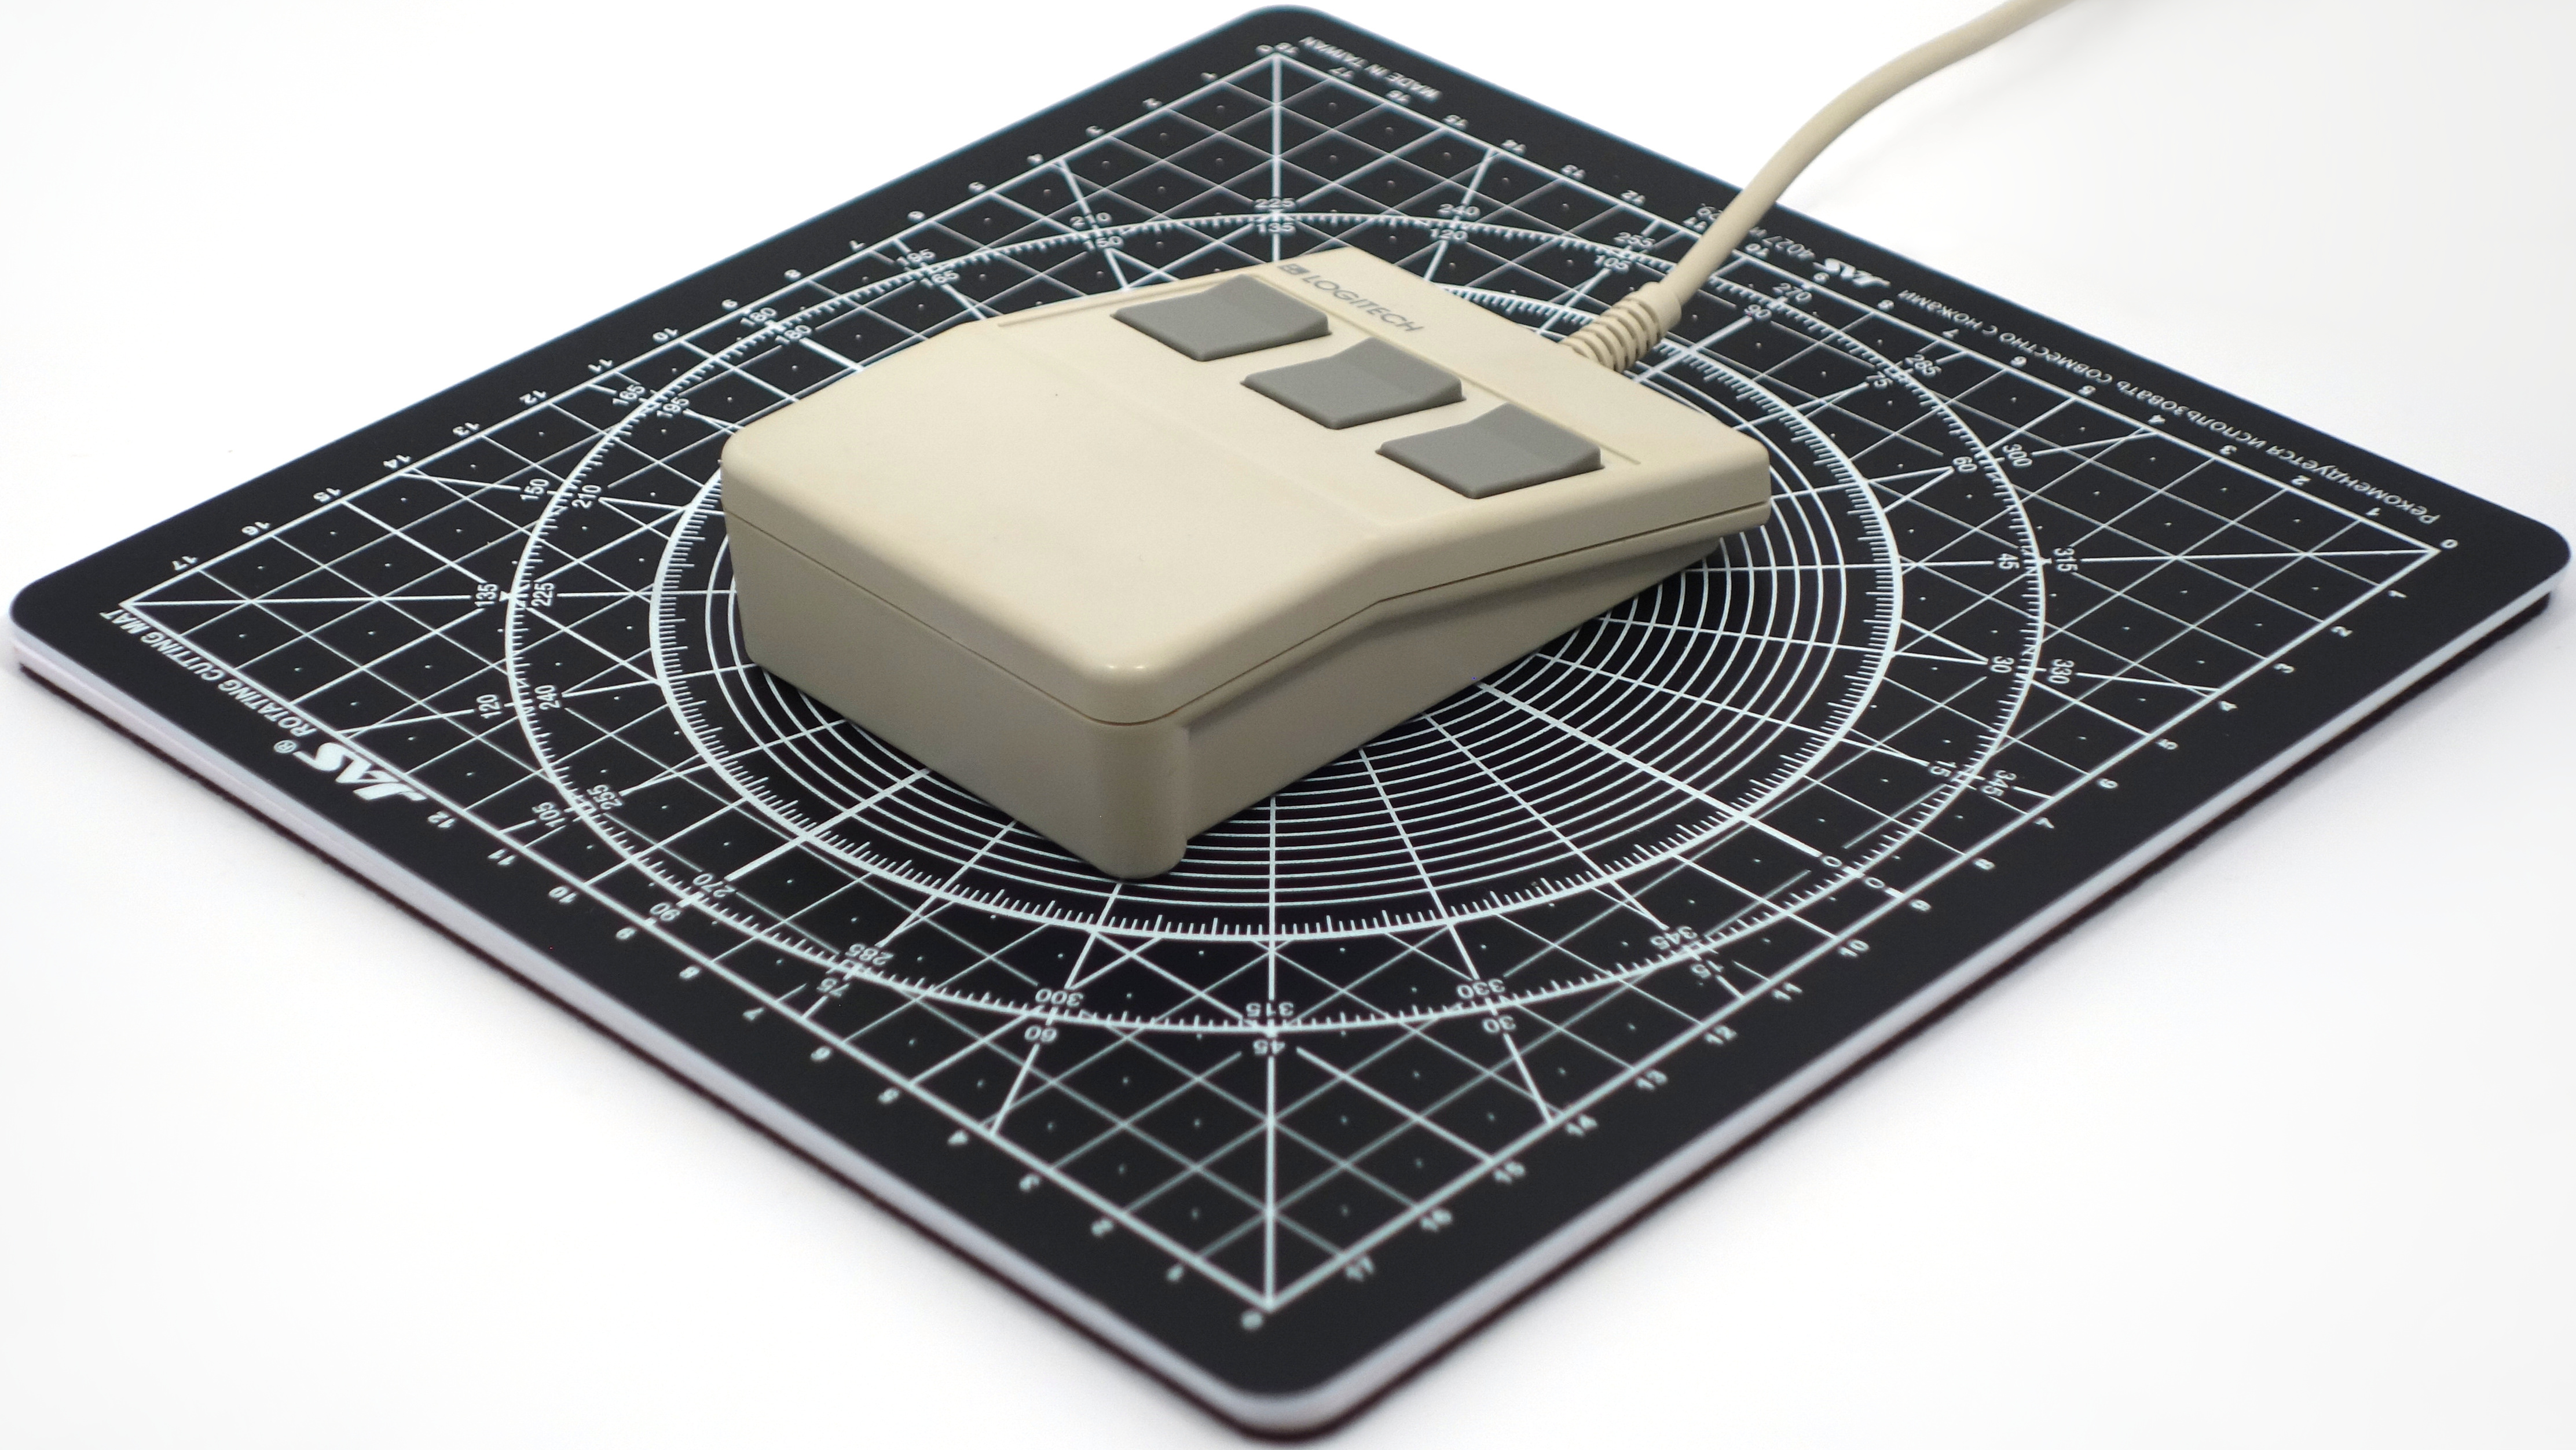
\includegraphics[scale=0.35]{1985_logitech_c7_mouse/size_30.jpg}
    \caption{Logitech C7 mouse на размерном коврике с шагом сетки 1~см}
    \label{fig:LogitechC7Size}
\end{figure}

Мышь имеет размеры, типичные для мышей 1980-х годов (рис. \ref{fig:LogitechC7Size}), не слишком отличающиеся от предыдущей модели, P5. Что касается эргономики, то очевидно, отказ от оригинального дизайна Антуана Каэна в пользу более прагматичного решения пошел ей на пользу. Верхняя часть корпуса предусматривает опору для ладони, а кнопки достаточно удобно нажимать палцами (рис. \ref{fig:LogitechC7Hand}). В начале 90-х угловатость C7 будет смотреться 
проигрышно в сравнении с мышами более обтекаемых форм, однако для середины 80-х годов мышь имеет неплохой уровень эргономики.

\begin{figure}[h]
    \centering
    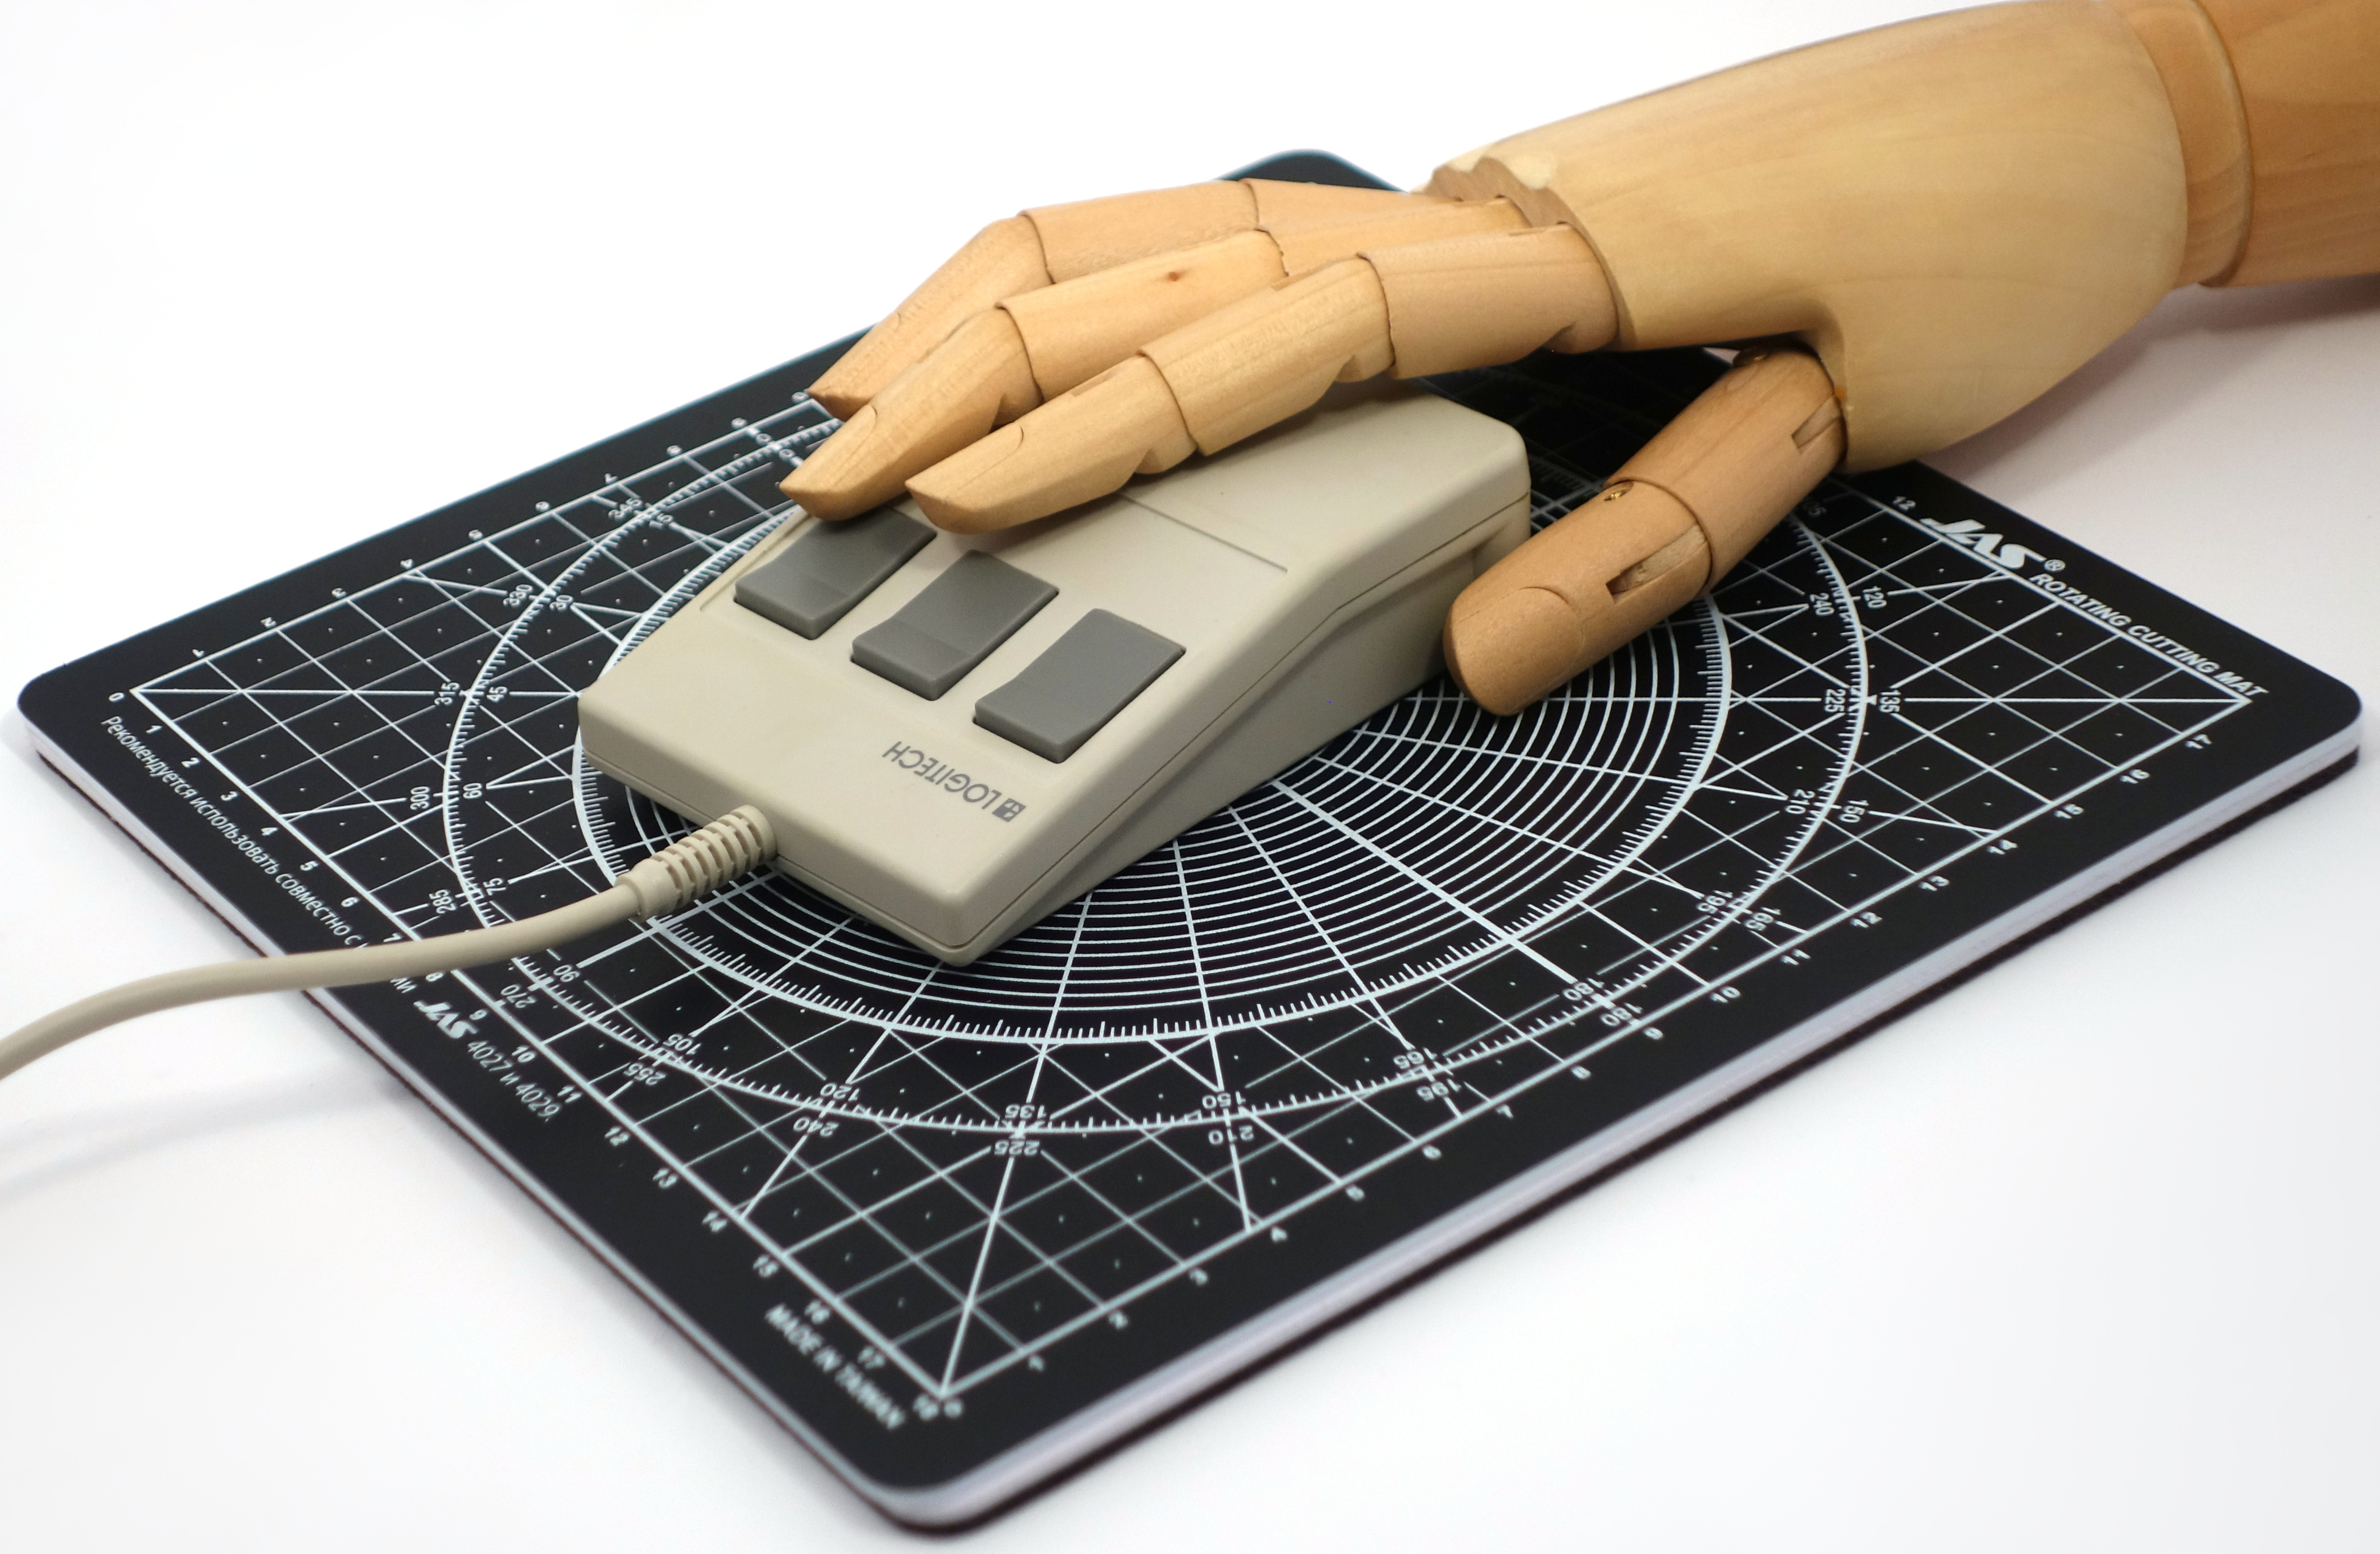
\includegraphics[scale=0.35]{1985_logitech_c7_mouse/hand_30.jpg}
    \caption{Logitech C7 mouse с моделью руки человека}
    \label{fig:LogitechC7Hand}
\end{figure}

Внутреннее устройство мыши показано на рис. \ref{fig:LogitechC7Inside}. Как и LOGIMOUSE P5, данная мышь является оптомеханической. Компоновка C7 также во многом повторяет P5, включая оптопары с оптическим прерывателем и весь механический узел. Среди отличий "---  отнести усложнившееся схемное решение (из-за использования последовательного интерфейса), ограничитель для защиты кабеля на выходе из корпуса, а также металлические пластины, которыми подпружиненны кнопки. Также следует отметить, что С7, вероятно, одна из первых мышей с интерфейсом RS-232, в которой были применены низкопотребляющие светодиоды и потому не требовалось внешнее питание (в случае P5 такой вопрос не был актуальным, поскольку квадратурный интерфейс в любом случае позволял получить достаточно мощности).

\begin{figure}[h]
    \centering
    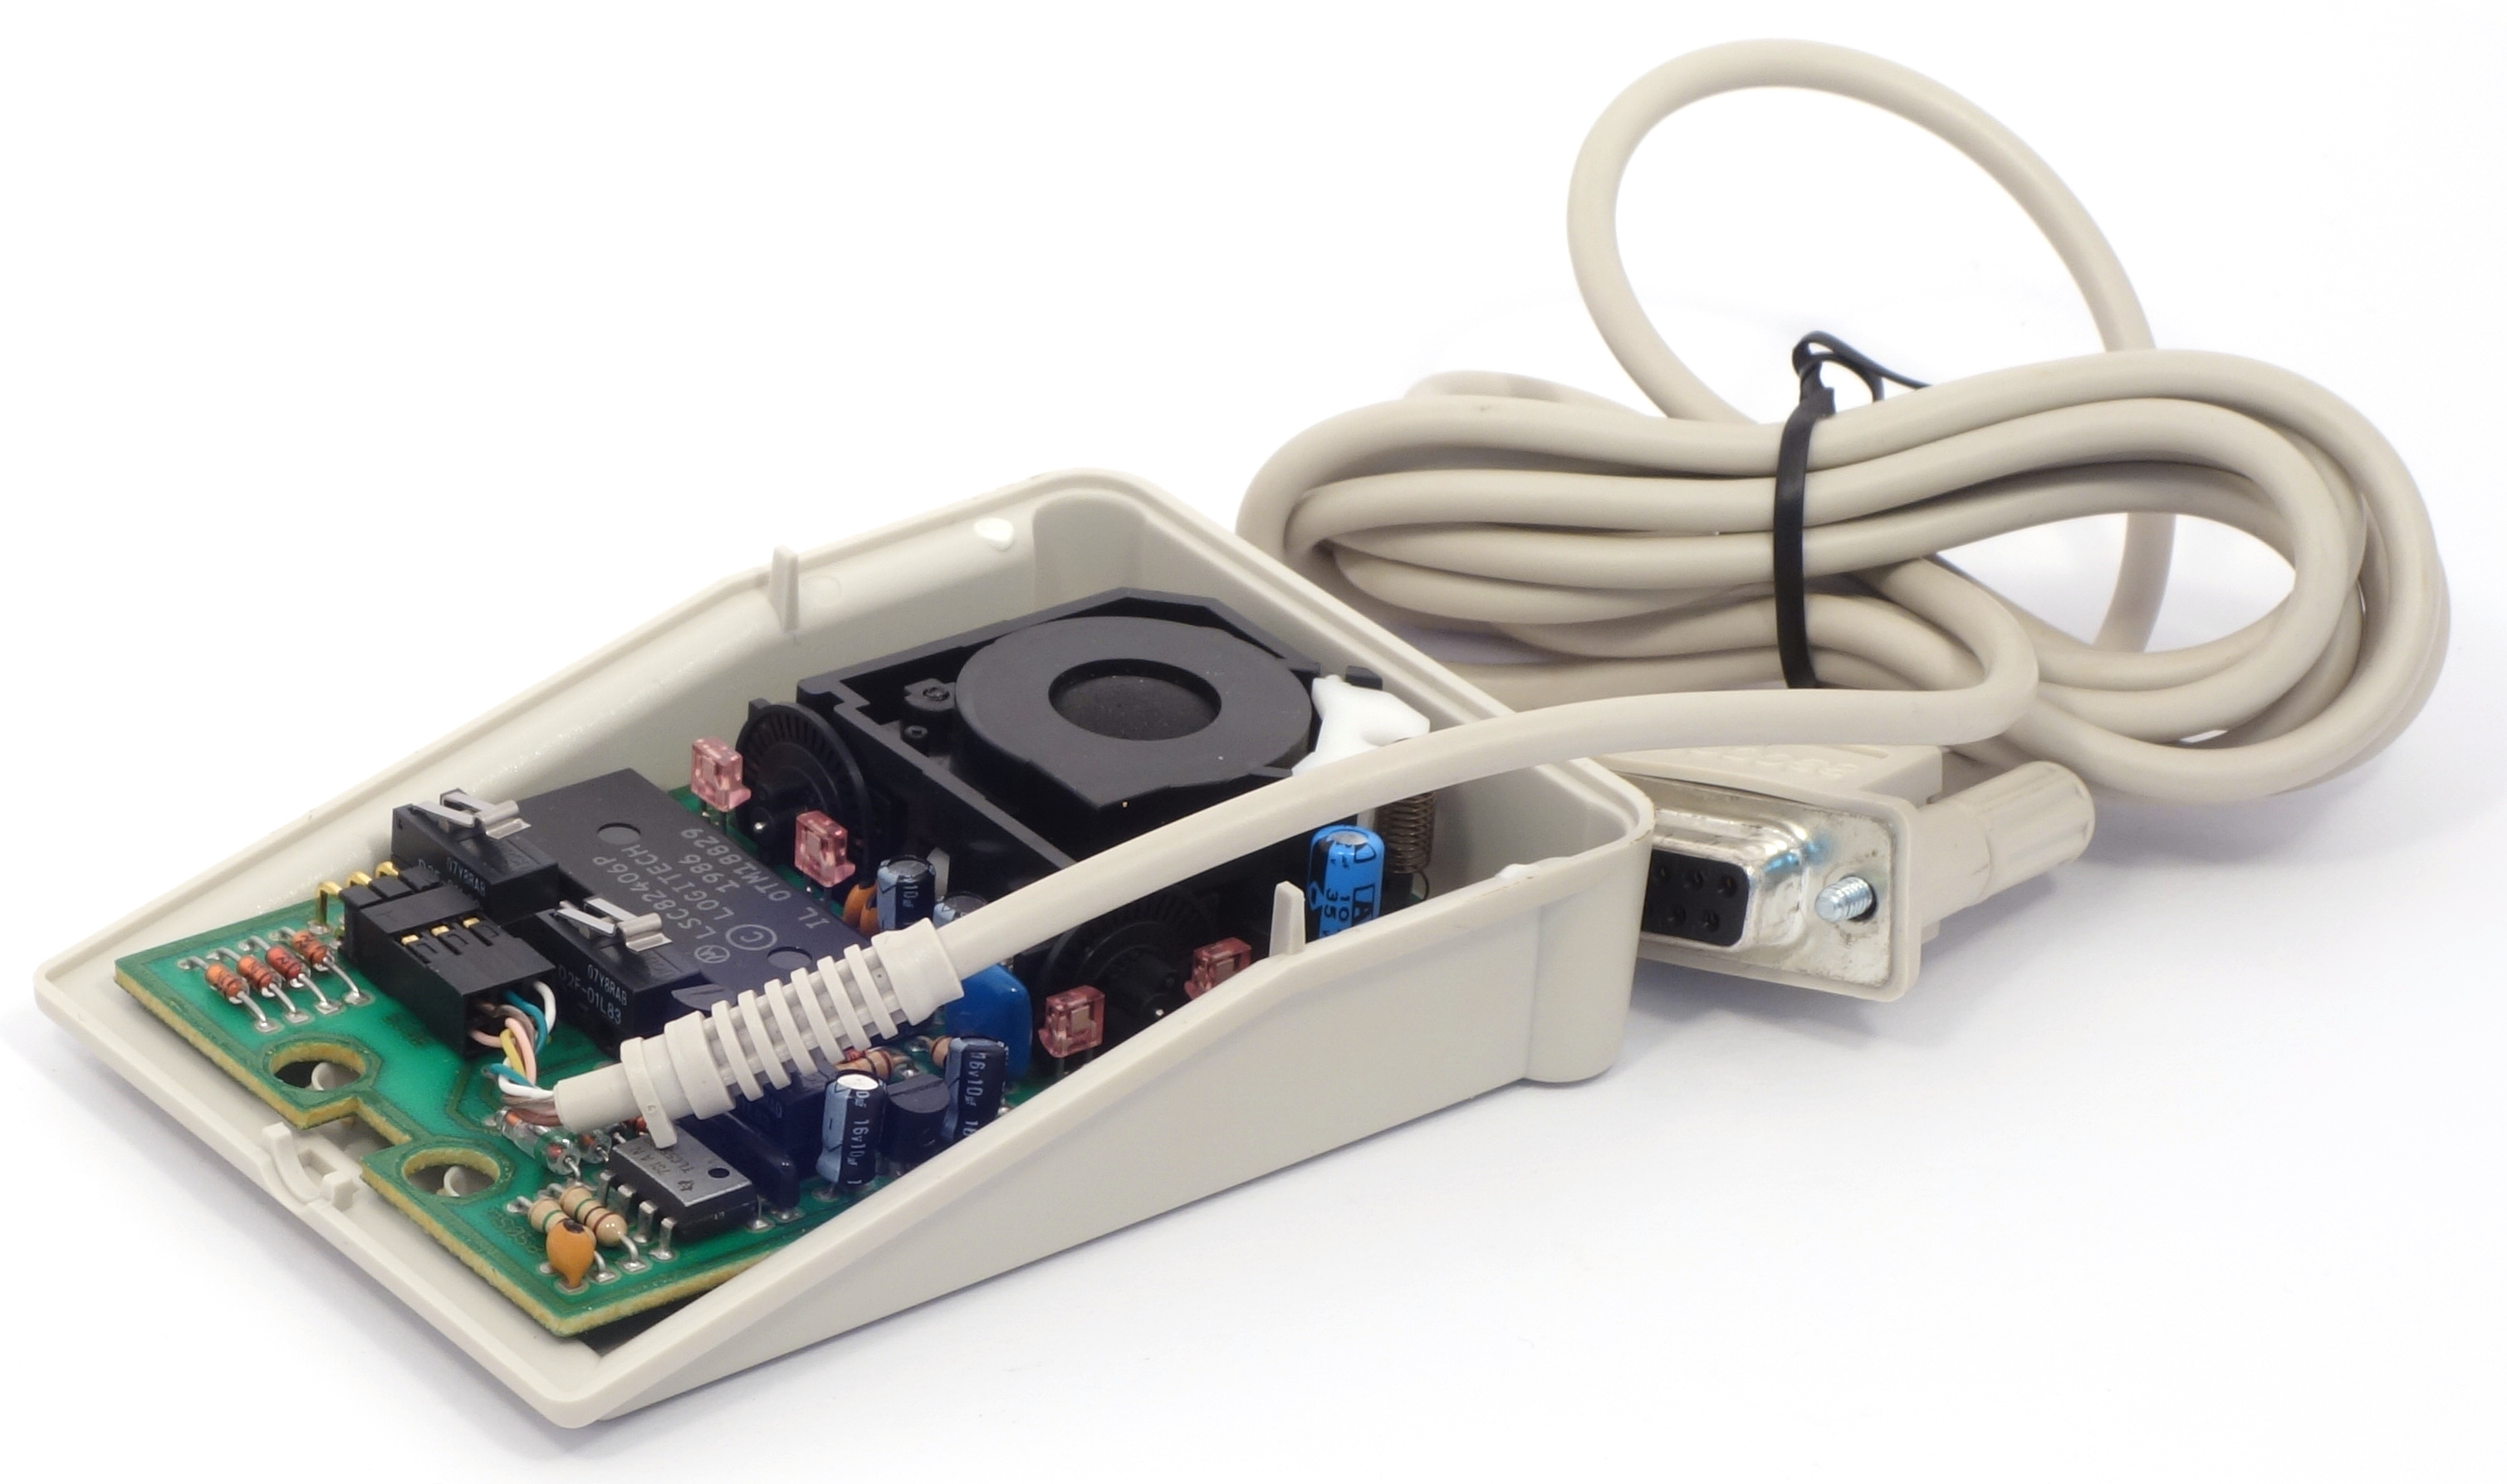
\includegraphics[scale=0.7]{1985_logitech_c7_mouse/inside_60.jpg}
    \caption{Logitech C7 mouse в разобранном виде}
    \label{fig:LogitechC7Inside}
\end{figure}

\begin{thebibliography}{9}
\bibitem {history} Logitech History. 2007 \url{https://web.archive.org/web/20081221120203/http://www.logitech.com/lang/pdf/logitech_history_200703.pdf}
\bibitem {timeline} Mouse timeline scroll by Logitech. Historic Firsts: The Mouse. Doug Engelbart Institute. \url{https://www.dougengelbart.org/content/view/162/#img1}
\bibitem {manual1} LOGIMOUSE C7 Technical Reference Manual. Firmware Revision 3.0. 1986. \url{https://bitsavers.org/pdf/logitech/mouse/Logitech_Logimouse_C7_Firmware_Rev_3.0_Jan86.pdf}
\bibitem {manual2} LOGITECH MOUSE User's Manual. Serial Mouse, Bus Mouse, Series 2 Mouse. 1987. \url{https://bitsavers.org/pdf/logitech/mouse/Logitech_Mouse_Users_Manual_Feb87.pdf}
\end{thebibliography}
\end{document}
